\section{PCE Maps} % {{{
\subsection{Quantum channels}
Quantum channels comprehend the most general linear operations that a quantum system undergo independently of its past
\subsection{Single qubit case} % {{{
% \ddnote{Sugiero otro nombre para esta seccion, pues los PCE no son los unicos
% mapas proyectivos, hay mapas proyectivos no unitales}
\todo{David escribe una primera version y luego Carlos itera}
\begin{itemize}
\item The single qubit case, describe some of the features.
\item Single qubit Kraus operators.
\item Single qubit relation with decoherence. 
\end{itemize}
% }}}
\subsection{Pauli component erasing maps} % {{{
\begin{itemize}
\item Give a formal definition of the PCE \todo{Jose Alfredo escribe}
\item Give some two qubit examples to illustrate non-trivial points with examples
(isualizacion y ejemplos)
\todo{Jose Alfredo escribe}
\item Canales de Ruskai Pauli maps, que la interseccion es no trivial (no estan contenidos en ninguna direccion, pero la interseccion es no vacia)
y Relación con canales citados en \cite{Siudzinska2020}? \cpnote{Esto quiza lo tengamos
que mover si es que necesitamos herramientas que discutiremos mas adelante para
hacer notar la diferencia}
\end{itemize}
% }}}
% \begin{itemize}
% \item Son positivas todas las matrices de densidad que resultan de aplicar un
% mapeo no válido? \janote{Creo que sí.  Para 1 qubit aplicar PCEs no CP siempre
% te deja dentro de la esfera de Bloch.  Así que estoy casi seguro que lo mismo
% sucede para $n$ qubits.}
% \end{itemize}
% }}}

The density matrix $\rho$ of a system of $n$ qubits can be written in Pauli matrices basis as 
\begin{equation}\label{eq:N_qubits_rho}
	\rho =\frac{1}{2^N} \sum_{j_1,\ldots,j_N=0}^3 \paulicomponents
	\sigma_{j_1}\otimes \ldots \otimes \sigma_{j_N},
	%r_{0,\ldots,0}=1,
\end{equation}
where $r_{0,\ldots,0}=1$ ($\Tr\rho=1$) and $\sigma_0=\openone$.
We may and will refer to $\paulicomponents$ as the ``Pauli components'' of the 
density matrix of a sistem of qubits. 

Let us now define a Pauli component erasing (PCE) operation. A linear operation 
$\mcE$ that acts on a density matrix $\rho$ of a system of qubits is a PCE operation if 
it transforms the Pauli components of $\rho$ as 
\begin{equation}
\begin{split}
	\paulicomponents \mapsto \ \taus \paulicomponents,\hspace{.5cm}\\
	\taus = 0,1, \hspace{1.5cm}	\tau_{0,\ldots,0}=1.
\end{split}
\end{equation}
A PCE operation is a trace-preserving operation that leaves invariant or erases 
the Pauli components of a density matrix of $n$ qubits. \janote{Ojo que aquí 
habrá que unificar la notación de subíndices. No lo hago porque no lo tengo del 
todo claro y no hay problema en dejarlo así por el momento.}

In \Fref{fig:PCE_figs} we introduce a pictorial representation of PCE operations of 
1, 2 and 3 qubits. Every position in the column, board or cube is associated with 
the subindices of $\taus$ of a PCE operation. If a little square or cube  in position
$j_1,\ldots,j_N$ is black, then $\taus=1$, if it is white, then $\taus=0$. For example,
\begin{center}
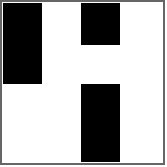
\includegraphics[width=2cm]{2qubits_pce_example}
\end{center}
this represents a PCE operation of 2 qubits that leaves invariant the Pauli 
components $r_{0,0}$, $r_{0,2}$, $r_{1,0}$, $r_{2,2}$, $r_{3,2}$. This operation
is not completely positive and therefore is not a quantum channel. In contrast, 
\begin{center}
\includegraphics[width=2cm]{2qubits_pceChannel_example01}
\end{center}
this other example of PCE operation that leaves invariant Pauli components 
$r_{0,0}$, $r_{1,2}$, $r_{2,1}$, $r_{3,3}$ satisfies complete positivity and 
is a quantum channel. 

\begin{figure} % {{{
	\centering
	\hfill \hfill
	\includegraphics[height=2.5cm]	{tablero_1qubit}
	\hfill
	\includegraphics[height=2.5cm]{tablero_2qubits}
	\hspace{1mm}
	\includegraphics[height=2.7cm]{rho-3q}
	\hfill \hfill
	\caption{From left to right representations of identity map
	(also PCE operations) of 1, 2 and 3 qubits, respectively.}
	\label{fig:PCE_figs}
\end{figure} % }}}

\begin{figure} % {{{
	\centering
	\includegraphics[height=2.5cm]	{1qubit_PCEChannels}
	\caption{1 qubit PCE channels. }
	\label{fig:1qubit_PCEChannles}
\end{figure} % }}}